\documentclass[../main.tex]{subfiles}
\graphicspath{{assets/}{../assets/}}

\begin{document}

    \section{Description générale du logiciel}
    \subsection{Environnement}

    \paragraph{}
    L’environnement dans lequel sera développé le moteur de recherche est le système d’exploitation Linux. Plus particulièrement, le développement se fera sous le langage C dans un premier temps. L’environnement doit alors supporter le langage C afin de faire fonctionner l’application sur la machine.

    \paragraph{}
    Nous retrouverons aussi l’utilisateur qui va pouvoir interagir avec les entrées (clavier…) et sorties du système (écran…) afin de communiquer avec le logiciel.

    \subsection{Composantes du logiciel et acteurs}

    \paragraph{}
    Une base de document est mise à disposition et contient des documents de type Texte, de type Image et de type Audio. Ainsi, il y aura une base de descripteurs pour chaque type de document traité, qui sauvegardera chaque descripteur.

    \paragraph{}
    Au sein de l’application, nous avons deux acteurs:
    \begin{itemize}
        \item L’\underline{utilisateur} doit pouvoir formuler une requête via le moteur de recherche et ainsi consulter le résultat de celle-ci.
        \item L’\underline{administrateur}, en plus d’hériter de toutes les fonctionnalités de l’utilisateur, doit pouvoir configurer le processus d’indexation, lancer l’indexation et visualiser les descripteurs.
    \end{itemize}

    \subsection{Fonctionnalités}
    \paragraph{}
    Le logiciel se décompose donc en deux grandes parties fonctionnelles:
    \begin{itemize}
        \item Une partie d’indexation.
        \item Une partie de comparaison.
    \end{itemize}

    \paragraph{}
    La dernière partie sera l'intégration des éléments précédents sous la forme d’un moteur de recherche qui comparera et triera les résultats en fonction de paramètres et de configurations pour ensuite afficher à l’utilisateur les documents les plus proches de la recherche.

    \paragraph{}
    Plusieurs types de documents sont pris en compte dans ce projet dans des extensions spécifiques (voir Tab~\ref{fig:ext_types}).  	

    \begin{table}[H]
        \centering
        \begin{tabular}{| c | c | c |}
            \hline
            \rowcolor{Gray}Type de document & Extension & Version .txt disponible \\
            \hline
            Texte & .xml & Non \\
            \hline
            Image couleur & .jpg & Oui (matrices intensités des pixels = RGB) \\
            \hline
            Image noir et blanc & .bmp & Oui (matrice intensités des pixels niveau de gris) \\
            \hline
            Audio & .wav .bin &  Oui (valeurs des échantillons du signal numérisé) \\
            \hline
        \end{tabular}

        \caption{Tableau récapitulatif des différents types de données pris en charge}
        \label{fig:ext_types}
    \end{table}

    % TO DO
    \paragraph{}
    Voici un diagramme des cas d’utilisation qui reprend toutes les fonctionnalités évoquées précédemment:

    \begin{figure}[h]
        \centering
        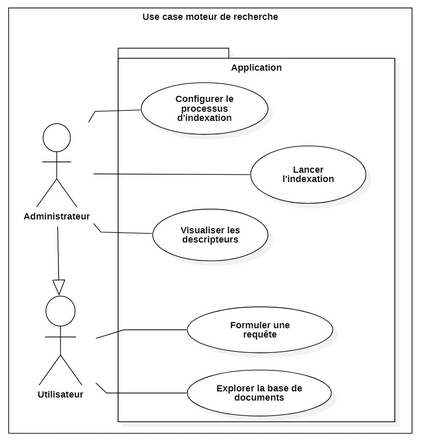
\includegraphics[width=100mm]{diagrams/user_interactions.png}
        \caption{Diagramme des cas d'utilisations (use case)}
    \end{figure}

\end{document}